\documentclass[a4paper]{article}

\usepackage[utf8]{inputenc}
\usepackage[T1]{fontenc}
\usepackage{textcomp}
\usepackage[english]{babel}
\usepackage{amsmath, amssymb}
\usepackage{natbib}
\usepackage{listings}
% figure support
\usepackage{import}
\usepackage{xifthen}
\pdfminorversion=7
\usepackage{pdfpages}
\usepackage{transparent}
\pdfsuppresswarningpagegroup=1

\title{Assignment 4}
\author{Linus Falk}
\begin{document}
\maketitle
\section*{WO 1.3}
\textbf{The following system of second order equations arises from studying the gravitational attraction of one mass by another. Convert it to a system of first order equations}

\begin{equation}
x(t)^{\prime \prime} = -\frac{cx(t)} {r(t)^{3}} \quad y(t)^{\prime \prime} = -\frac{cy(t)} {r(t)^{3}}  \quad z(t)^{\prime \prime} = -\frac{cz(t)} {r(t)^{3}}  
\end{equation}

\textbf{with} 

\begin{equation}
r(t) = \sqrt{x(t)^{2}+y(t)^{2}+z(t)^{2}}
\end{equation}

let v denote the system of equations $v =[x, x^{\prime}, y, y^{\prime},z, z^{\prime} ] $ and let $v_1^{\prime} = v_2, v_2^{\prime} = -\frac{-v_1c} {r(t)^{3}}$ and so on. We then end up with the system of equations below: 

\begin{equation}
 \begin{bmatrix} v_1 \\ v_2 \\v_3 \\v_4 \\v_5 \\v_6 \end{bmatrix}^{\prime} = \begin{bmatrix} v_2 \\ \frac{v_1c} {r^{3}} \\ v_4 \\ \frac{v_3c} {r^{3}}  \\ v_6 \\ \frac{v_5c} {r^{3}}   \end{bmatrix} = \begin{bmatrix} v_2 \\ \frac{v_1c} {(x(t)^{2}+y(t)^{2}+z(t))^{\frac{3} {2} }} \\ v_4 \\ \frac{v_3c} {x(t)^{2}+y(t)^{2}+z(t)^{\frac{3} {2} }}  \\ v_6 \\ \frac{v_5c} {(x(t)^{2}+y(t)^{2}+z(t))^{\frac{3} {2} }}   \end{bmatrix}
 \end{equation} 

The system can now be solved with RK4 for example. 

\newpage

\section*{WO 1.5}
\textbf{For the chemical reaction model (1.9) show that for $K_1 \neq K_2$ the general solution of the ODE is}
\begin{equation}
y_j = cj_ e^{-K_1t} + c_2e^{-K_2t}+c_{j3} \quad j=1,2,3
\end{equation}
\textbf{For some constants $c_{1j}$,$c_{2j}$ and $c_{3j}$. Let $y_1(0)$,$y_2(0)$ and $y_3(0)$ be initial values. Show that $y_1$ decay exponentially to 0. If $K_1 > K_2$ show $y_2$ grows first but ultimately decay to zero. But $y_3$ grows and asymptotically approaches the value $y_1(0)$+$y_2(0)$+$y_(0)$. Plot the graph solutions for values $K_1 = 3$ and $K_2 = 1$}
\\
\\
The chemical reaction can be described as $A \overset{K_1}{\rightarrow} B \overset{K_2}{\rightarrow}C$. Let $y_1 = A$, $y_2 = B$ and $y_3 = C$. Then we can formulate the ode's for the reaction and the initial condition. 

\begin{equation}
\begin{aligned}
y_1^{\prime} = -K_1 y_1 \\
y_2^{\prime} = K_1 y_1 - K_2 y_2\\
y_3 ^{\prime} = K_2 y_2 \\
\\
y(0) = y_1(t) + y_2(t) + y_3(t)
\end{aligned}
\end{equation}



Examining the process we can see that concentration of A is decaying to 0 and that the concentration of C is going to be the sum of the initial value of A and B (A and B decays to C). If we take a look on $y_1$ we know the solution: 

\begin{equation}
\begin{aligned}
y_1 = y(0) e^{-K_1 t} \\
\\
y_2^{\prime} = y_1(0) e^{-K_1 t} - K_2y_2 \\
y_3^{\prime} = K_2y_2
\end{aligned}
\end{equation}

by the method of integrating factor we can solve $y_2$

\begin{equation}
\begin{aligned}
y_2^{\prime} e^{K_2t} + K_2y_2e^{K_2t} = y(0) e^{-K_1 t}e^{K_2t} = K_1y(0) e^{(K_2-K_1)t} \\
y_2^{\prime}e^{K_2t} = K_1 y(0)e^{(K_2-K_1)t}
\end{aligned}
\end{equation}

Now integrating both sides and rearrange

\begin{equation}
\begin{aligned}
y_2 e^{K_2t} = \frac{1} {K_2-K_1} K_1 y(0) e^{(K_2-K_1)t} + y(0) \\
y_2 = \frac{K_1} {K_2-K_1} y(0) e^{-K_1t}+ y(0) e^{-K_2t}
\end{aligned}
\end{equation}

Put this result into $y_3^{\prime}$ and we get:

\begin{equation}
\begin{aligned}
y_3^{\prime}  = K_2y_2 = \frac{K_1K_2} {K_2-K_1} y(0) (e^{-K_1t}+ e^{-K_2t})
\end{aligned}
\end{equation}

But since we now that the decay is balanced we can conclude that: \\ $C = y(0) - y_1 - y_2$

\begin{equation}
\begin{aligned}
y_3 = y(0) - y(0) e^{-K_1 t} - \frac{K_1} {K_2-K_1} y(0) (e^{-K_1t}+ e^{-K_2t}) \\
y_3 = y(0) \begin{bmatrix}1- e^{-K_1 t} -  \frac{K_1} {K_2-K_1}(e^{-K_1t} + e^{-K_2t})  \end{bmatrix}
\end{aligned}
\end{equation}

Putting it all together gives: 

\begin{equation}
\begin{aligned}
\begin{bmatrix} y_1 \\ y_2 \\ y_3 \end{bmatrix} = \begin{bmatrix} y(0) e^{-K_1 t}  \\ y(0)\begin{bmatrix} \frac{K_1} {K_2-K_1}(e^{-K_1t}+  e^{-K_2t}) \end{bmatrix}\\ y(0) \begin{bmatrix}1- e^{-K_1 t} -  \frac{K_1} {K_2-K_1}(e^{-K_1t} + e^{-K_2t})  \end{bmatrix}\end{bmatrix}
\end{aligned}
\end{equation}



\section*{WO 2.1}
\textbf{Generalize the error analysis of the Euler's method for system of IVP $y^{\prime} = f(t,y(t))$ with $y(t_0) = y_0$}

\section{WO 2.8}
\textbf{Let $\Theta \in \begin{bmatrix} 0, 1 \end{bmatrix}$ and denote $t_{k+\Theta} = (1-\Theta)t_k+t_\Theta{k+1}$. Consider the generalized midpoint method}
\begin{equation}
y_{k+1} = y_k+hf(t_{k+\Theta},(1-\Theta)y_k+\Theta y_{k+1})
\end{equation}
\textbf{and the generalized trapezoidal method}
\begin{equation}
y_{k+1} = y_k+h \begin{bmatrix} (1-\Theta)f(t_k,y_k) + \Theta f(t_{k+1},t_{k+1})  \end{bmatrix}
\end{equation}

\textbf{Determine the absolute stability region of this methods. Separate the cases $\Theta \in [0,1/2)$ and $ \Theta \in \begin{bmatrix} 1/2,1 \end{bmatrix}$}


For midpoint we use the test equation: $w = \lambda y$ 

\begin{equation}
\begin{aligned}
y_{k+1} = y_k + h()
\end{aligned}
\end{equation}


For generalized trapezoidal method we use the test equation again: $w = \lambda y$ 



\begin{equation}
 \begin{aligned}
 y_{k+1} = y_k+ w\begin{bmatrix} (1-\Theta)y_k + \Theta y_{k+1}  \end{bmatrix}\\
 y_{k+1} = y_k+ w(1-\Theta)y_k + w\Theta y_{k+1}\\
 y_{k+1}(1 - w \Theta ) = y_k + w(1 -  \Theta)y_k \\
 y_{k+1} = y_k \frac{(1 + w(1 - \Theta))} {(1 - w \Theta )} 
 \end{aligned}
\end{equation}

The stability region is therefore

\begin{equation}
 w \in C : \frac{(1 + w(1 - \Theta))} {(1 - w \Theta )}  < 1
\end{equation}


\section*{WO 2.13}
\textbf{Write down the equations for RK4 method for solving linear system of equations $y^{\prime}(t) = Ay(t)$ with initial condition y(0) = y0}

\begin{equation}
\begin{aligned}
Ay = \begin{bmatrix} a_{11}& a_{12}& \ldots& a_{1n} \\
                    a_{21}& a_{22}& \ldots& a_{2n} \\
                    \vdots& \vdots& \vdots& \vdots \\
                    a_{m1}& a_{m2}& \ldots& a_{mn} \end{bmatrix} 
                    \begin{bmatrix} y_1 \\ y_2\\ \vdots \\ y_n \end{bmatrix}
\end{aligned}
\end{equation}

\begin{equation}
\begin{bmatrix} f_1 \\ f_2 \\ \vdots \\ f_n  \end{bmatrix} =
\begin{bmatrix} a_{11}y_1 + a_{12}y_2 + \ldots + a_{1n}y_n \\
                a_{21}y_1 + a_{22}y_2 + \ldots + a_{2n}y_n \\
                \vdots \\
                a_{m1}y_1 + a_{m2}y_2 + \ldots + a_{mn}y_n \\
                 \end{bmatrix}
\end{equation}

\begin{equation}
\begin{aligned}
k1_1 = f_1 \\
k2_1 = f_1 +  \frac{k2_1} {2} \\
k3_1 = f_1 +  \frac{k2_1} {2} \\
k4_1 = f_1 +  k3_1 \\
y1_{i+1} = f_1 + \frac{1} {6}(k1_1 + 2k2_1 + 2k3_1 + k4_1) \\
\quad \vdots \quad \quad \quad \quad \quad \vdots \quad \quad \quad \quad  \quad \vdots \\
k1_n = f_n \\
k2_n = f_n +  \frac{k2_n} {2} \\
k3_n = f_n +  \frac{k2_n} {2} \\
k4_n = f_n +  k3_n \\
yn_{i+1} = f_1 + \frac{1} {6}(k_n + 2k2_n + 2k3_n + k4_n) 
\end{aligned}
\end{equation}


\section*{WO 2.22}



\section*{Python 2.12}
\begin{lstlisting}[language=Python]
def analytic2(t):
    return t/(1+t**2)


def RK2(t0, y0, tn, n):
    h = (tn - t0) / n
    res = []
    for j in range(n):
        k1 = h * f(t0, y0)
        k2 = h * f(t0 + h/2, y0 + k1/2)

        yn = y0 + k2
        res.append(yn)
        y0 = yn
        t0 = t0 + h
    return res


def RK3(t0, y0, tn, n):
    h = (tn - t0) / n
    res = []
    for j in range(n):
        k1 = h * f(t0, y0)
        k2 = h * f(t0 + 0.5 * h, y0 + 0.5 * k1)
        k3 = h * f(t0 + h,  y0 + 2 * k2 - k1)

        yn = y0 + (1.0/6.0) * (k1 + 4*k2 + k3)

        res.append(yn)

        y0 = yn
        t0 = t0 + h
    return res


def RK4(t0, y0, tn, n):
    h = (tn - t0) / n
    res = []
    for j in range(n):
        k1 = h * (f(t0, y0))
        k2 = h * (f((t0 + h / 2), (y0 + k1 / 2)))
        k3 = h * (f((t0 + h / 2), (y0 + k2 / 2)))
        k4 = h * (f((t0 + h), (y0 + k3)))
        k = (k1 + 2 * k2 + 2 * k3 + k4) / 6

        yn = y0 + k

        res.append(yn)

        y0 = yn
        t0 = t0 + h
    return res


stp = []
s = 0.2
for x in range(6):
    stp.append(s)
    s = s/2


result1=[]; result2=[]; result3=[]
analyticres = []
logscale = []

result_1 = []

for k in range(len(stp)):
    tn = 1
    t0 = 0
    y0 = 0
    n = int((tn - t0) / stp[k])
    result1.append(math.log(abs(RK2(t0, y0, tn, n)[-1] - 0.5)))
    result2.append(math.log(abs(RK3(t0, y0, tn, n)[-1] - 0.5)))
    result3.append(math.log(abs(RK4(t0, y0, tn, n)[-1] - 0.5)))
    logscale.append(math.log(stp[k]))

print('RK2 order of convergence: ', (result1[-1]-result1[0])/(logscale[-1]-logscale[0]))
print('RK3 order of convergence: ', (result2[-1]-result2[0])/(logscale[-1]-logscale[0]))
print('RK4 order of convergence: ', (result3[-1]-result3[0])/(logscale[-1]-logscale[0]))

plt.plot(logscale, result1, label='RK3')
plt.plot(logscale, result2, label='RK3')
plt.plot(logscale, result3, label='RK4')
plt.legend()
plt.show()

OUTPUT :
RK2 order of convergence:  2.0784386063625684
RK3 order of convergence:  3.005946020526148
RK4 order of convergence:  4.070616072356785

\end{lstlisting}

\begin{figure}[ht!]
\centering
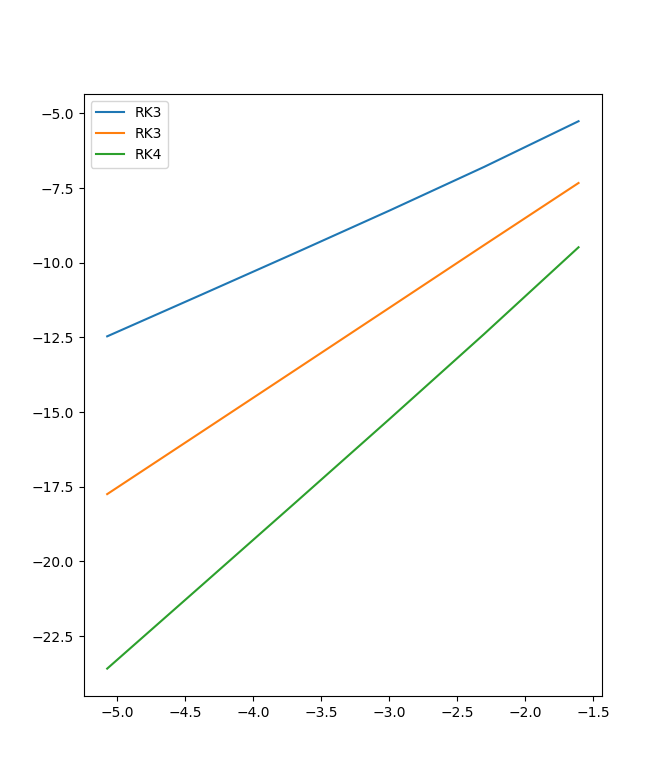
\includegraphics[scale=0.5]{Figure_1.png}
\caption{RK2,3,4 convergence }
\label{fig:dig}
\end{figure}


\begin{lstlisting}[language=Python]
import matplotlib.pyplot as plt
import numpy as np
from numpy.linalg import inv, norm
import math


def func(x):
   return np.sin(np.pi*x)


def analytic(t,x):
    return np.exp(-t*np.pi**2)*np.sin(np.pi*x)


def generateA(m):
    A = np.eye(m)
    for i in range(m-1):
        A[i][i] = -2
        A[i+1][i] = 1
        A[i][i+1] = 1
    A[-1][-1] = -2
    return A


def trap(x, h):
    I = np.eye(1001)
    A = generateA(1001)
    A = (1/0.001**2) * A
    return inv(I-h/2*A)@(h/2*A+I)@x


def BDFq3(t, h, y, y_1, y_2): #Now implicit Euler
    A = generateA(1001)
    A = (1/0.001**2)*A
    return inv(np.eye(1001) - 6 / 11 * h * A) @ (18 / 11 * y - 9 / 11 * y_1 + 2 / 11 * y_2)



'''defining the space'''
deltaX = 0.001
xline = np.arange(0, 1+deltaX, deltaX)


'''step size in time'''
stp = []; h = 0.2
for x in range(6):
    stp.append(h)
    h = h/2

'''intital values'''
t0 = 0
tn = 1
y = func(xline)
y[0] = 0
y[-1] = 0

dt = stp[0]
n = int((tn/dt))
D = dt/(deltaX**2)


y1 = trap(y, dt)
y2 = trap(y1, dt)
buff = y
y = y2
y2 = buff
lst = [y, y1, y2]

t = 0
a = analytic(t, xline)
t = t + dt

errorlist = []
logstep = []
for y in range(len(stp)):
    dt = stp[y]
    print(dt)
    y = func(xline)
    y[0] = 0
    y[-1] = 0

    y1 = trap(y, dt)  # change to RK2 steps when done
    y2 = trap(y1, dt)  # change to RK2 steps when done
    buff = y
    y = y2
    y2 = buff
    lst = [y, y1, y2]

    t = 0
    for x in range(2,int(tn/dt), 1):
        lst.append(BDFq3(t0, dt, lst[x], lst[x-1], lst[x-2]))
        a = analytic(t, xline)
        t = t + dt
    print(norm(lst[-1]-a))
    errorlist.append(math.log(norm(lst[-1]-a)))
    logstep.append(math.log(dt))

plt.plot(logstep, errorlist)
err = round((errorlist[-1]-errorlist[0])/(logstep[-1]-logstep[0]), 4)
plt.grid()
plt.title('Order of convergence: ' + str(err))
plt.xlabel('log(h)')
plt.ylabel('log(norm(error))')
plt.show()


print('Order of convergence: ', (errorlist[-1]-errorlist[0])/(logstep[-1]-logstep[0]))


OUTPUT: Order of convergence:  2.9311540109514937
\end{lstlisting}


\begin{figure}[ht!]
\centering
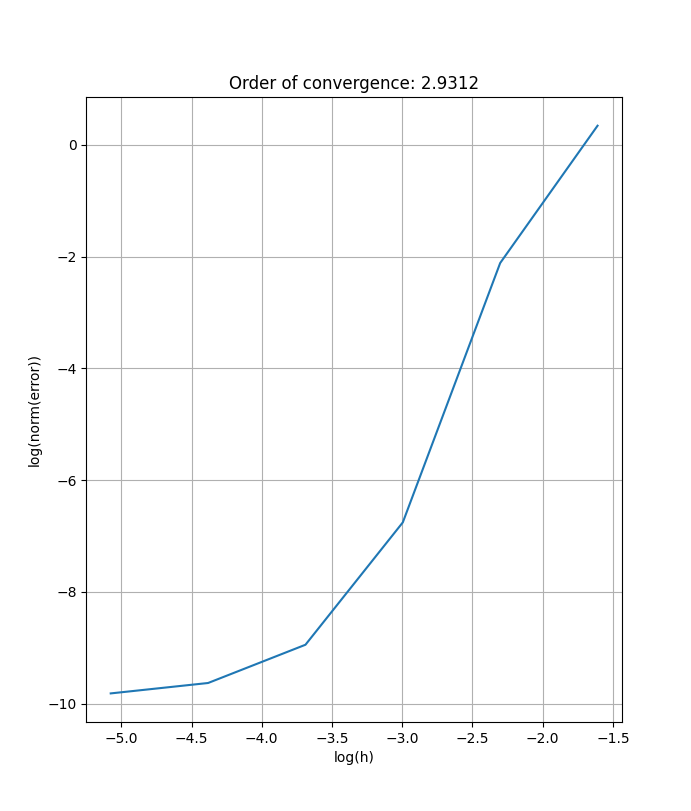
\includegraphics[scale=0.5]{Figure_2.png}
\caption{Order of convergence BDF3}
\label{fig:dig}
\end{figure}





\bibliographystyle{unsrt}
\bibliography{references}
\end{document}